\documentclass{article}%
\usepackage{amsmath}%
\usepackage{amsfonts}%
\usepackage{amssymb}%
\usepackage{graphicx}
\usepackage{amsthm}
\usepackage{enumitem}
%-------------------------------------------
\newtheorem{theorem}{Theorem}
\newtheorem{acknowledgement}[theorem]{Acknowledgement}
\newtheorem{algorithm}[theorem]{Algorithm}
\newtheorem{axiom}[theorem]{Axiom}
\newtheorem{case}[theorem]{Case}
\newtheorem{claim}[theorem]{Claim}
\newtheorem{conclusion}[theorem]{Conclusion}
\newtheorem{condition}[theorem]{Condition}
\newtheorem{conjecture}[theorem]{Conjecture}
\newtheorem{corollary}[theorem]{Corollary}
\newtheorem{criterion}[theorem]{Criterion}
\newtheorem{definition}[theorem]{Definition}
\newtheorem{example}[theorem]{Example}
\newtheorem{exercise}[theorem]{Exercise}
\newtheorem{lemma}[theorem]{Lemma}
\newtheorem{notation}[theorem]{Notation}
\newtheorem{problem}[theorem]{Problem}
\newtheorem{proposition}[theorem]{Proposition}
\newtheorem{remark}[theorem]{Remark}
\newtheorem{solution}[theorem]{Solution}
\newtheorem{summary}[theorem]{Summary}

\theoremstyle{definition}
\newtheorem{question}{Question}


\setlength{\textwidth}{7.0in}
\setlength{\oddsidemargin}{-0.35in}
\setlength{\topmargin}{-0.5in}
\setlength{\textheight}{9.0in}
\setlength{\parindent}{0.3in}
\begin{document}

\begin{flushright}
\textbf{Name: KimJaeHwan\hspace{0.1cm} \;\\
Student ID: 20230499\hspace{0.35cm} }
\end{flushright}

\begin{center}
\textbf{CSED261: Discrete Mathematics for Computer Science \\
Homework 5: Number Theory and Cryptography} \\
\end{center}

\begin{question}
Prove or disprove that if $A, B$ and $C$ are nonempty sets and $A \times B = A \times C$, then $B = C$.
\end{question}

\par\noindent\rule{\textwidth}{0.5pt}

\subsubsection*{Solutions}
\indent
I'll use proof by contradiction.
Let $B = {b_0, b_1, \cdots b_n}$ and $C = {c_0, c_1, \cdots c_m}$.
Let's assume that $A \times B = A \times C$ however $B \neq C$.
Without the generality, Let $a_0 \in A$, and $b_0 \in B$ and $b_0 \notin C$ or vice versa. Then, $(a_0, b_0) \in A \times B$ but $(a_0, b_0) \notin A \times C$. So, $A \times B \neq A \times C$, this is a contradiction.

\newpage
\begin{question}
Compare the number of comparisons used by the insertion sort and the binary insertion sort to sort the list 7, 4, 3, 8, 1, 5, 4, 2.
\end{question}

\par\noindent\rule{\textwidth}{0.5pt}

\subsubsection*{Solutions}

Insertion sort (Ascending order)
\smallskip

\begin{tabular}{|c|c|c|}
    \hline
    Input & 7, 4, 3, 8, 1, 5, 4, 2& Comparison \\
    \hline
    Step 1& ((4, 7)), 3, 8, 1, 5, 4, 2& (4, 7) change \\
    \hline
    Step 2& (4, (3, 7)), 8, 1, 5, 4, 2& (3, 7) change\\
    Step 2& ((3, 4), 7), 8, 1, 5, 4, 2& (3, 4) change\\
    \hline
    Step 3& (3, 4, (7, 8)), 1, 5, 4, 2& (7, 8) no-change\\
    \hline
    Step 4& (3, 4, 7, (1, 8)), 5, 4, 2& (1, 8) change\\
    Step 4& (3, 4, (1, 7), 8), 5, 4, 2& (1, 7) change\\
    Step 4& (3, (1, 4), 7, 8), 5, 4, 2& (1, 4) change\\
    Step 4& ((1, 3), 4, 7, 8), 5, 4, 2& (1, 3) change\\
    \hline
    Step 5& (1, 3, 4, 7, (5, 8)), 4, 2& (5, 8) change\\
    Step 5& (1, 3, 4, (5, 7), 8), 4, 2& (5, 7) change\\
    Step 5& (1, 3, (4, 5), 7, 8), 4, 2& (4, 5) no-change\\
    \hline
    Step 6& (1, 3, 4, 5, 7, (4, 8)), 2& (4, 8) change\\
    Step 6& (1, 3, 4, 5, (4, 7), 8), 2& (4, 7) change\\
    Step 6& (1, 3, 4, (4, 5), 7, 8), 2& (4, 5) change\\
    Step 6& (1, 3, (4, 4), 5, 7, 8), 2& (4, 4) no-change\\
    \hline
    Step 7& (1, 3, 4, 4, 5, 7, (2, 8))& (2, 8) change\\
    Step 7& (1, 3, 4, 4, 5, (2, 7), 8)& (2, 7) change\\
    Step 7& (1, 3, 4, 4, (2, 5), 7, 8)& (2, 5) change\\
    Step 7& (1, 3, 4, (2, 4), 5, 7, 8)& (2, 4) change\\
    Step 7& (1, 3, (2, 4), 4, 5, 7, 8)& (2, 4) change\\
    Step 7& (1, (2, 3), 4, 4, 5, 7, 8)& (2, 3) change\\
    Step 7& ((1, 2), 3, 4, 4, 5, 7, 8)& (1, 2) no-change\\
    \hline
\end{tabular}

\bigskip
\noindent Binary insertion sort (Ascending order)
\smallskip

\begin{tabular}{|c|c|c|}
    \hline
    Input & 7, 4, 3, 8, 1, 5, 4, 2& Comparison \\
    \hline
    Step 1& 7 & Initial input \\
    \hline
    Step 2& 4, 7 & (4, 7) compare (mid : 4)\\
    \hline
    Step 3& 3, 4, 7& (4, 3) compare (mid : 4)\\
    \hline
    Step 4& 3, 4, 7, 8& (4, 8) compare (mid : 4)\\
    Step 4& 3, 4, 7, 8& (7, 8) compare (mid : 7)\\
    \hline
    Step 5& 1, 3, 4, 7, 8& (4, 1) compare (mid : 4)\\
    Step 5& 1, 3, 4, 7, 8& (3, 1) compare (mid : 3)\\
    \hline
    Step 6& 1, 3, 4, 5, 7, 8& (4, 5) compare (mid : 4)\\
    \hline
    Step 7& 1, 3, 4, 4, 5, 7, 8& (4, 4) compare (mid : 4)\\
    \hline
    Step 8& 1, 2, 3, 4, 4, 5, 7, 8& (4, 2) compare (mid : 4)\\
    Step 8& 1, 2, 3, 4, 4, 5, 7, 8& (3, 2) compare (mid : 3)\\
    \hline
\end{tabular}

\bigskip
\textbf{Conclusion} : The number of comparisons used by the insertion sort is 22 and the number of comparisons used by the binary insertion sort is 11. The binary insertion sort is faster than the insertion sort.
\newpage
\begin{question}
Show that each of these pairs of functions are of the same order.
\begin{enumerate}
    \item $3x+7, x$
    \item $\log (x^2+1), \log_2x$
\end{enumerate}
\end{question}

\par\noindent\rule{\textwidth}{0.5pt}

\subsubsection*{Solutions}
\begin{enumerate}
    \item $3x+7, x$
    Generally, we can use limit of the ratio of two functions to show that pairs of functions are of the same order

    $$\lim_{x \to \infty} \frac {3x + 7} x = 3$$

    Since the limit is a (nonw-zero) constant, $3x+7$ and $x$ are of the same order.

    \item $\log (x^2+1), \log_2x$
    Let's use same method.

    $$\lim_{x \to \infty} \frac {\log (x^2+1)} {\log_2x} = \lim_{x \to \infty} \frac {\log (x^2+1)} {\frac {\log x} {\log 2}} = \lim_{x \to \infty} \frac {\log (x^2+1)} {\log x} \cdot \log 2$$

    To compute the limit of fraction having log in numerator and denominator, we can use L'Hopital's rule:

    $$\lim_{x \to \infty} \frac {f(x)} {g(x)} = \lim_{x \to \infty} \frac {f'(x)} {g'(x)}$$

    So we get:

    $$\lim_{x \to \infty} \frac {\log (x^2+1)} {\log x} = \lim_{x \to \infty} \frac {\frac {2x} {x^2+1}} {\frac 1 x} = \lim_{x \to \infty} \frac {2x^2} {x^2+1} = 2$$

    So, the limitation of ratio of two functions is a non-zero constant, $2\log 2$, so $\log (x^2+1)$ and $\log_2x$ are of the same order.
\end{enumerate}
\newpage
\begin{question}
Prove that $\sum_{j=1}^n j(j+1)(j+2) \cdots(j+k-1)=n(n+1)$ $(n+2) \cdots(n+k) /(k+1)$ for all positive integers $k$ and n. [Hint: Use a technique from Exercise 33]


\begin{figure}[h!]
    \centering
    \fbox{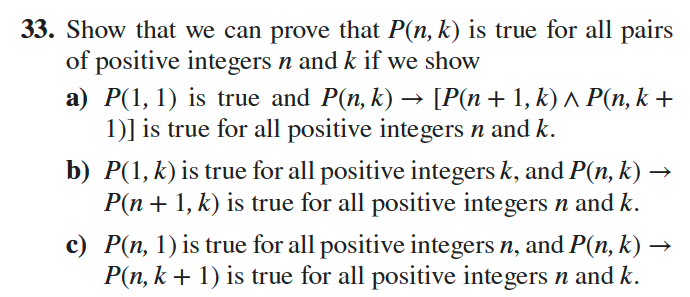
\includegraphics[width=0.5\linewidth]{questions/Exer33.png}}
\end{figure}

\end{question}

\par\noindent\rule{\textwidth}{0.5pt}

\subsubsection*{Solutions}

\begin{proof}
    Let $P(n, k)$ be the statement $\sum_{j=1}^n j(j+1)(j+2) \cdots(j+k-1)=n(n+1)$ $(n+2) \cdots(n+k) /(k+1)$ for all positive integers $k$ and n. We will prove that $P(n, k)$ is true for all pairs of positive integers $n$ and $k$ by induction on $n$ and $k$ followinng the step $b$ of Exercise 33.\\
    \textbf{Base Case:} \\
    $P(1, k) \Longleftrightarrow \sum_{j=1}^1 j(j+1)(j+2) \cdots(j+k-1) = 1(1+1)(1+2) \cdots(1+k-1) = 1 = 1(1+1)(1+2) \cdots(1+k)/(k+1)$ is true for all positive integer $k$.\\
    \begin{align*}
        P(n+1, k) \Longleftrightarrow & \sum_{j=1}^{n+1} j(j+1)(j+2) \cdots(j+k-1) \\
        = &\sum_{j=1}^{n} j(j+1)(j+2) \cdots(j+k-1) + (n+1)(n+2) \cdots(n+k)\\
        = & \frac {n(n+1) \cdots(n+k)} {k+1} + (n+1)(n+2) \cdots(n+k) & \because \text{$P(n, k)$ is true}\\
        = & \frac {n(n+1) \cdots(n+k) + (n+1)(n+2) \cdots(n+k)(k+1)} {k+1}\\
        = & \frac {(n+1)(n+2) \cdots(n+k)(n+k+1)} {k+1} & \text{So, $P(n+1, k)$ is true}
    \end{align*}
    Therefore, by induction, $P(n, k)$ is true for all positive integers $n$ and $k$.
\end{proof}
\newpage
\begin{question}
Find the strongly connected components of each of these graphs.

\begin{figure}[htb!]
  \centering
  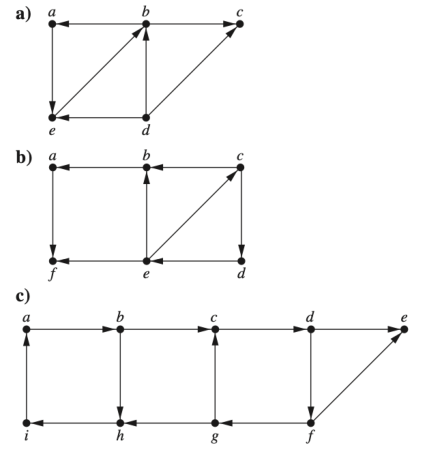
\includegraphics[width=0.4\linewidth]{q5_figure.pdf}
\end{figure}

\end{question}

\par\noindent\rule{\textwidth}{0.5pt}

\subsubsection*{Solutions}
\begin{enumerate}[label=\textbf{\alph*).}]
  \item (a, b, e), (d), (c)
  \item (a), (f), (b), (c, d, e)
  \item (a, b, c, d, f, g, h, i), (e)

\end{enumerate}
\newpage
\begin{question}
How many of the disjunctions $p \lor \neg q$, $\neg p \lor q$, $q \lor r$, $q \lor \neg r$, and $\neg q \lor \neg r$ can be made simultaneously true by an assignment of truth values to $p$, $q$, and $r$?
\end{question}

\par\noindent\rule{\textwidth}{0.5pt}

\subsubsection*{Solutions}

\begin{center}
\begin{tabular}[h]{|ccc|ccccc|r|}
    \hline
    p & q & r & $p \lor \neg q$ & $\neg p \lor q$ & $q \lor r$ & $q \lor \neg r$ & $\neg q \lor \neg r$ & correct \\
    \hline
    T & T & T & T & T & T & T & F & 4 \\
    T & T & F & T & T & T & T & T & 5 \\
    T & F & T & T & F & T & F & T & 3 \\
    T & F & F & T & F & F & T & T & 3 \\
    F & T & T & F & T & T & T & F & 3 \\
    F & T & F & F & T & T & T & T & 4 \\
    F & F & T & T & T & T & F & T & 4 \\
    F & F & F & T & T & F & T & T & 4 \\
    \hline
\end{tabular}
\end{center}

\noindent So, when $(p, q, r) = (T, T, F)$, all of the disjunctions can be true simultaneously. Therefore, the answer is \textbf{5}.
\end{document}